\section{Проектирование}

Этот раздел содержит описание теоретических аспектов работы.
В первую очередь здесь будет детально рассмотрена
структура информационных моделей,
используемых как источник исходных данных для визуализации.
Далее идет описание клиентской и серверной части прототипа,
описание проблем, которых это разделение призвано решить,
а также описание функциональности, которую они будут предоставлять.
Наконец, эта глава также содержит кратких обзор методик,
используемых для повышения производительности визуализации.

\subsection{Описание предметной области}

Далее рассматривается структура информационной модели.
В связи с тем, что в качестве целевого формата был выбран  формат Revit,
дальнейшее описание предметной области будет в первую очередь
соответствовать стандартам Autodesk Revit.
Различия с другими форматами, например Industry Foundation Classes (IFC-формат),%
\cite{BuildingSmartIFC}
рассматриваться не будут.

\begin{figure}[h]
    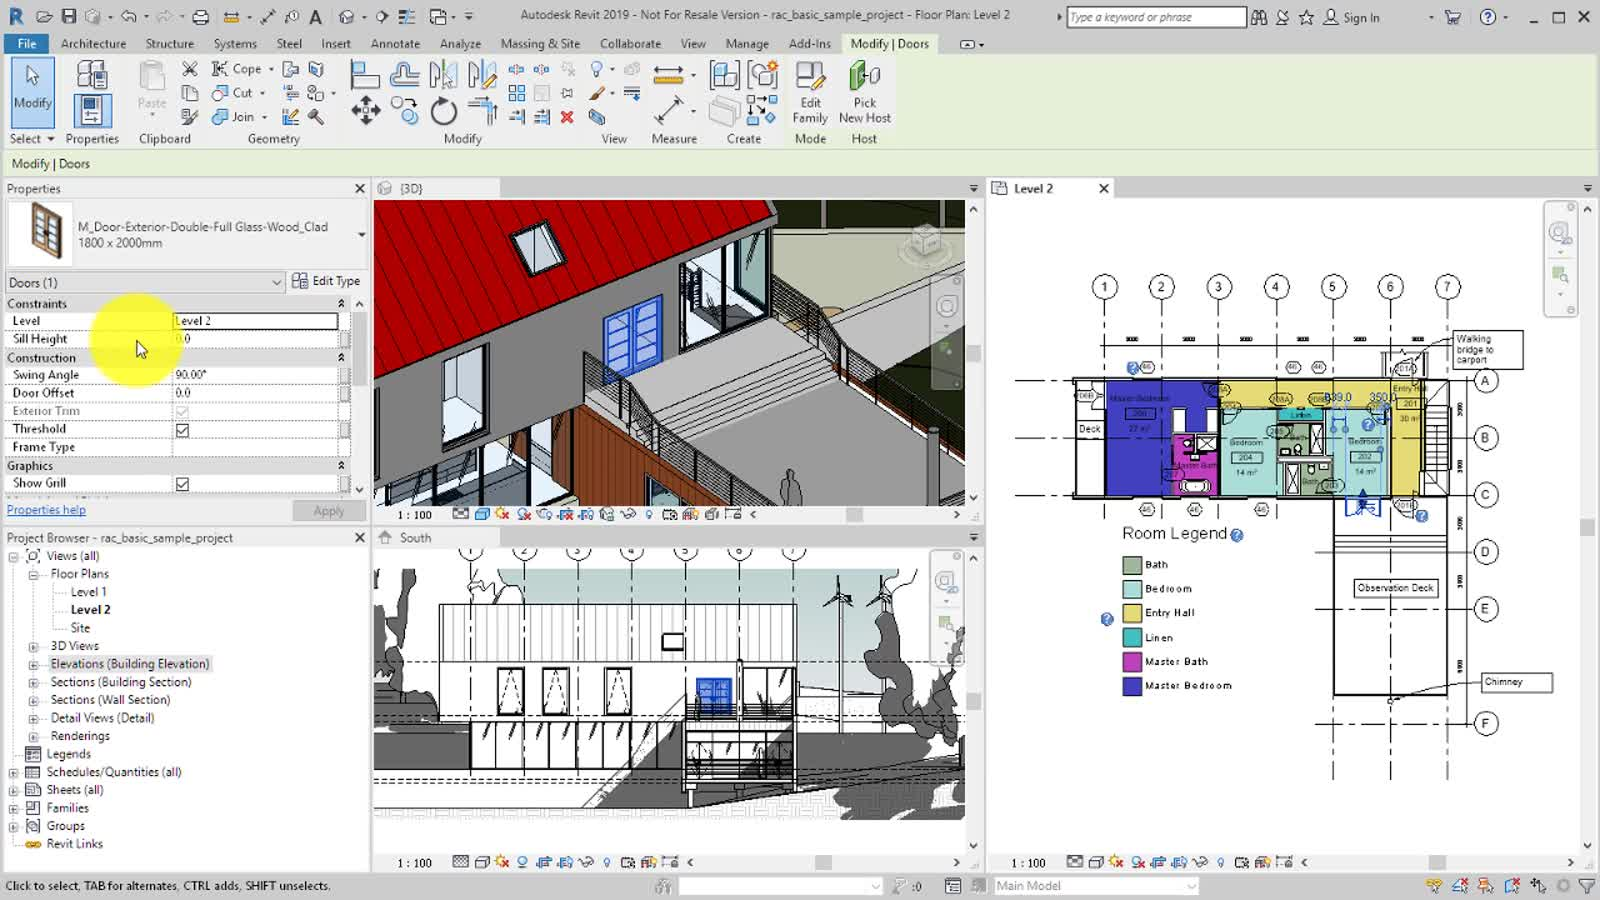
\includegraphics[width=\textwidth]{images/Revit-interface.jpg}
    \caption{Интерфейс редактора Revit}
    \label{figure:RevitInterface}
\end{figure}

Для хранения данных Revit использует специальный проприетарные форматы RVT, RFA и RTE.
Для отображения данных модели в виртуальной среде необходимо
преобразовывать их в форматы трехмерной графики, например OBJ или FBX.

\paragraph{Элементы информационной модели}

Каждая сущность в проекте информационной модели называется элементом.
Revit использует 3 типа элементов в проектах:
элементы модели, опорные элементы и элементы, относящиеся к представлению.
Элементы в Revit также часто называются семействами.
Семейство содержит геометрическое определение элемента и
параметры, используемые элементом.
Каждый экземпляр элемента определяется и контролируется семейством.%
\cite{DocRevit}
Для создания визуализации нас в первую очередь интересуют
именно элементы модели.

\begin{figure}[h]
    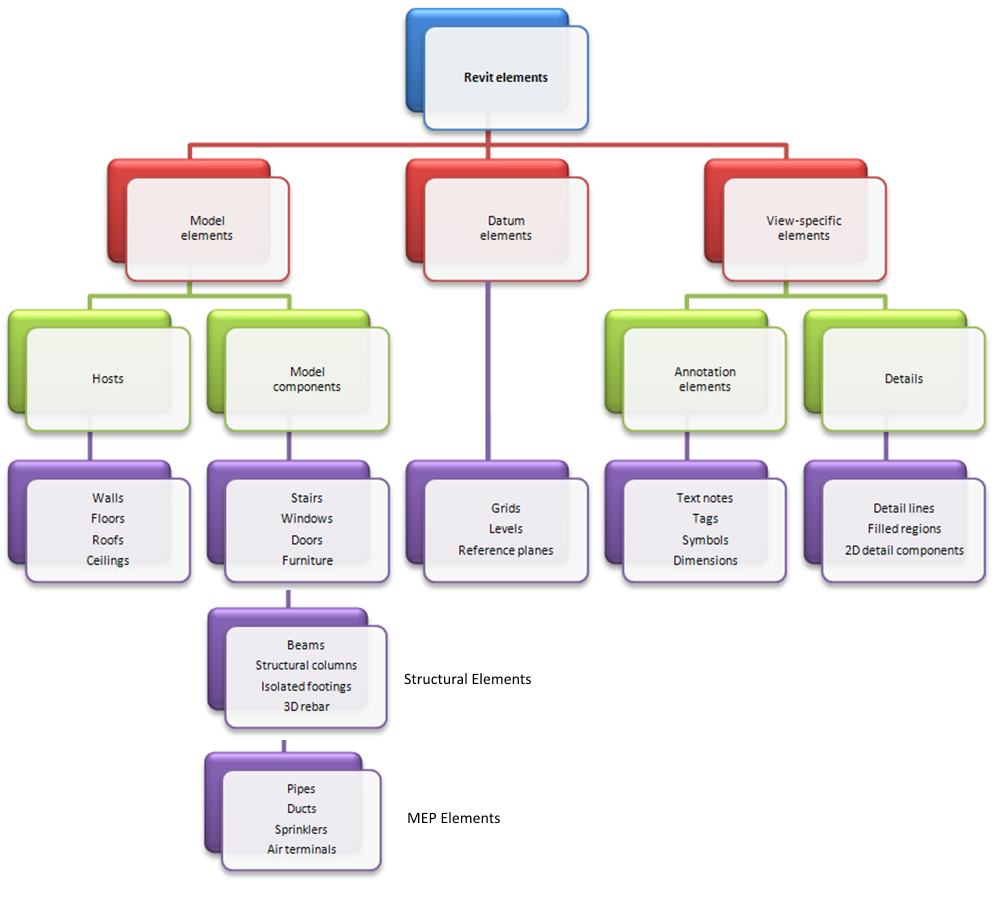
\includegraphics[width=\textwidth]{images/Revit-elements.png}
    \caption{Элементы информационной модели}
    \label{figure:RevitElements}
\end{figure}

\subparagraph{Элементы модели:}

Элементы модели представляют фактическую трехмерную геометрию здания,
например стены, окна, двери, пандусы,
воздуховоды и электрические панели.
Элементы модели делятся на хосты и компоненты модели.
Хостами обычно являются элементы,
которые возводятся непосредственно на строительной площадке,
например стены и потолки.
Компонентами модели являются все остальные типы элементов модели.

\subparagraph{Опорные элементы:}

Опорные элементы помогают определить контекст проекта.
К ним относятся опорные плоскости, уровни и сетки.

\subparagraph{Элементы представления:}

Элементы представления это элементы,
отображаемые только в каком-то определенном режиме представления проекта.
Они помогают описывать или документировать модель.

\paragraph{Свойства элементов}

Каждый размещаемый элемент является экземпляром семейства.
Элементы имеют 2 набора свойств, управляющих их внешним видом и поведением:
свойства типа и свойства экземпляра.%
\cite{DocRevit}

\subparagraph{Свойства типа:}

Один и тот же набор свойств типа является общим для всех элементов семейства,
и каждое свойство имеет одинаковое значение для всех экземпляров определенного типа семейства.
Изменение значения свойства типа влияет на все текущие и будущие экземпляры этого семейства.

\subparagraph{Свойства экземпляра:}

Общий набор свойств экземпляра также применяется ко всем элементам,
принадлежащим к определенному типу семейства,
но значения этих свойств могут различаться.
Например, размеры окна являются свойствами типа,
а его высота над уровнем пола является свойством экземпляра.


\subsection{Описание структуры клиентской и серверной части}

Теперь можно поподробнее рассмотреть архитектуру прототипа.
Как было сказано ранее, основное предназначение приложения~--~
презентация информационной модели участникам проекта,
не имеющим навыков моделирования,
например заказчикам, спонсорам или непосредственным пользователям здания.
Такая презентация поможет успешнее вносить
корректировки в проект еще на самых ранних стадиях,
что снизит финальные затраты на реализацию проекта.%
\cite{Davidson2019}

Исходя из описанных требований можно сделать вывод о том,
что конечные пользователи приложения не станут использовать
программное обеспечение информационного моделирования.
Для них имеют значение только финальные или промежуточные результаты работы.
Поэтому было принято решение отделить функциональность приложения,
взаимодействующую с исходными данными модели.
Клиентская часть может не зависеть
от конкретной системы информационного моделирования,
что упростит расширение системы в дальнейшем.
Так же это может повысить производительность визуализации в клиентской части,
так как все трудоемкие вычисления, проводимые над исходными данными,
можно проводить на серверной части.

\paragraph{Функциональность серверной части}

Далее представлена основная функциональность реализуемая прототипом на "сервере".

\begin{enumerate}
    \item {
        Хранение исходной информационной модели.
        Сервер должен хранить исходную модель,
        а также распознавать ее изменения для повторного преобразования.
    }
    \item {
        Конвертация формата RVT в формат FBX.
        Поскольку формат данных информационной модели отличается от
        представления классических форматов трехмерной графики
        и не поддерживается большинством фреймворков
        создания интерактивных графических приложений
        вроде Unity и Unreal, необходимо производить
        преобразование формата.
    } 
    \item {
        Предоптимизация модели.
        Из-за комплексности трехмерных моделей,
        получаемых после конвертации,
        необходимо проводить их дополнительную оптимизацию.
        Подробнее это будет рассмотрено в следующем разделе.
    }
    \item {
        Упаковка моделей.
        Оптимизированные модели должны упаковываться для
        загрузки в клиентской части приложения.
    }
\end{enumerate}

\paragraph{Функциональность клиентской части}

\intextcomment{
    Дополнительное описание и раскрытие пунктов списка!
}

\begin{enumerate}
    \item {
        Загрузка готовой модели.
        Приложение должно загружать выбранную упакованную модель.
        Так как в рамках прототипа не производится реализация удаленного сервера,
        загрузка будет происходить локально, как показано на рисунке~%
        \ref{figure:CModelLoader}.

        \begin{figure}[h]
            \centering
            \includegraphics[width=\textwidth*6/10]{example-image}
            \caption{Загрузчик моделей}
            \label{figure:CModelLoader}
        \end{figure}

        \intextcomment{
            Описание UML-схемы...
        }
    } 
    \item {
        Размещение модели в виртуальной среде.
        После загрузки модель должна размещаться в виртуальной сцене.
        Для визуализации будет использоваться виртуальный стол,
        на который будет проецироваться модель здания
        в уменьшенном масштабе согласно схеме на рисунке~%
        \ref{figure:CStand}.

        \begin{figure}[h]
            \centering
            \includegraphics[width=\textwidth*6/10]{example-image}
            \caption{Размещение модели}
            \label{figure:CStand}
        \end{figure}

        \intextcomment{
            Описание UML-схемы...
        }
    } 
    \item {
        Взаимодействие с элементами модели.
        После размещения модель будет разбивать на слои,
        представляющие отдельные структурные элементы здания,
        например стены, лестницы или двери.
        На каждый отдельный слой может накладываться эффект,
        изменяющий его отображение.
        На рисунке~\ref{figure:CLayers} показана
        структура системы слоев.

        \begin{figure}[h]
            \centering
            \includegraphics[width=\textwidth*6/10]{example-image}
            \caption{Система слоев}
            \label{figure:CLayers}
        \end{figure}

        \intextcomment{
            Описание UML-схемы...
        }
    } 
\end{enumerate}

\comment{
    TODO:

    Запилить UML!
}


\subsection{Оптимизационные подходы}

\lipsum[6]

\paragraph{Причины проблем с производительностью}

\lipsum[6]

\paragraph{Существующие подходы}

\lipsum[6]

\paragraph{Реализуемый подход}

\lipsum[6]

\comment{
    TODO:

    - вступление
        можно написать о важности оптимизации,
        т.к. при больших/сложных моделях фпс падает в нулину
    - Причины проблем с производительностью
        много полигонов
        много draw call'ов
    - Существующие подходы
        LOD
        Batching
        Culling
    - Реализуемый подход
        описать, что я слепливаю меши через 3ds max 

    тут можно набрать инфы
        https://docs.google.com/document/d/1UFfMFDzLpAvTebCliWfk5ZwtrGVYgcodpkItyuvP6hA/edit
}
